\documentclass[11pt,a4paper]{article}

% ==============================================================================
% PACKAGE IMPORTS
% ==============================================================================
\usepackage[utf8]{inputenc}
\usepackage[margin=0.95in]{geometry}
\usepackage{amsmath,amssymb}
\usepackage{booktabs,tabularx,multirow,array}
\usepackage{graphicx}
\usepackage{tikz}
\usetikzlibrary{shapes.geometric, arrows.meta, positioning, calc}
\usepackage{algorithm}
\usepackage{algpseudocode}
\usepackage{hyperref}
\usepackage{cite}
\usepackage{enumitem}
\usepackage{microtype}
\usepackage{fancyhdr}
\usepackage{setspace}
\usepackage{caption}
\usepackage{xcolor}

% ==============================================================================
% COLOR DEFINITIONS & HYPERLINK SETUP
% ==============================================================================
\definecolor{primaryblue}{RGB}{26, 86, 219}
\definecolor{darkslate}{RGB}{30, 41, 59}
\definecolor{lightgraybg}{RGB}{248, 250, 252}

\hypersetup{
    colorlinks=true,
    linkcolor=primaryblue,
    citecolor=primaryblue,
    urlcolor=primaryblue,
    pdftitle={Smart Document Scanner: Project Report},
    pdfauthor={Saurabh Kumar Singh, Shubhranshu Mishra, Shivanshu Mishra, Suresh Choudhary}
}

% ==============================================================================
% HEADER AND FOOTER CONFIGURATION
% ==============================================================================
\pagestyle{fancy}
\fancyhf{}
\fancyhead[L]{\small\textcolor{darkslate}{\textbf{Smart Document Scanner: IPCV Project Report}}}
\fancyhead[R]{\small\textcolor{darkslate}{Dr. Abhimanyu Sahu}}
\fancyfoot[C]{\thepage}
\renewcommand{\headrulewidth}{0.4pt}
\renewcommand{\footrulewidth}{0.4pt}

\setstretch{1.14}

% ==============================================================================
% DOCUMENT BEGINS
% ==============================================================================
\begin{document}

% ==============================================================================
% PAGE 1: COVER / TITLE PAGE
% ==============================================================================
\begin{titlepage}
    \centering
    \vspace*{1.0cm}

    {\Large \textbf{\textcolor{darkslate}{DEPARTMENT OF COMPUTER SCIENCE AND ENGINEERING}}}\\[0.4em]
    {\large \textbf{IMAGE PROCESSING AND COMPUTER VISION (IPCV)}}\\[2.0cm]

    \rule{\linewidth}{1.5pt}\\[1.0em]
    {\LARGE \textbf{\textcolor{primaryblue}{SMART DOCUMENT SCANNER:}}}\\[0.5em]
    {\Large \textbf{Automated Document Boundary Detection, Rotated Extrema Quad Extraction, and Planar Perspective Rectification}}\\[0.8em]
    \rule{\linewidth}{1.5pt}\\[2.5cm]

    \textbf{A CAPSTONE PROJECT REPORT SUBMITTED IN PARTIAL FULFILLMENT}\\[0.3em]
    \textbf{OF THE REQUIREMENTS FOR THE DEGREE OF}\\[0.3em]
    \textbf{BACHELOR OF TECHNOLOGY}\\[3.0cm]

    \begin{minipage}[t]{0.48\textwidth}
        \flushleft
        \textbf{\large Submitted to:}\\[0.4em]
        {\Large \textbf{Dr. Abhimanyu Sahu}}\\[0.2em]
        Faculty Evaluator / Mentor\\
        Department of Computer Science and Engineering
    \end{minipage}
    \hfill
    \begin{minipage}[t]{0.48\textwidth}
        \flushright
        \textbf{\large Submitted by (Team Members):}\\[0.4em]
        \textbf{Saurabh Kumar Singh} \quad (20233256)\\[0.25em]
        \textbf{Shubhranshu Mishra} \quad (20233272)\\[0.25em]
        \textbf{Shivanshu Mishra} \quad (20233267)\\[0.25em]
        \textbf{Suresh Choudhary} \quad (20233281)
    \end{minipage}

    \vfill
    {\large \textbf{Academic Year 2025--2026}}\\[0.3em]
    \today
\end{titlepage}

% ==============================================================================
% PAGE 2: ABSTRACT, TABLE OF CONTENTS & INTRODUCTION
% ==============================================================================
\newpage
\setcounter{page}{2}

\begin{abstract}
\noindent Digitizing paper media through mobile smartphone cameras routinely introduces strong perspective foreshortening, non-uniform cast illumination, and background clutter from desktops and surrounding objects. While commercial scanning applications often deploy heavy, non-explainable deep learning models that require significant memory footprints and lack deterministic auditability, this project presents \textbf{SmartScan}: an explainable, real-time, sub-60 millisecond document scanning and perspective rectification system engineered purely using classical Image Processing and Computer Vision (IPCV) principles. 

The core engineering contribution centers on resolving the fundamental failure modes of traditional edge detectors: (1) internal printed text interference is eliminated using non-destructive morphological closing ($17 \times 17$ rectangular kernel) without blurring outer paper perimeters; (2) a multi-modal segmentation ensemble combines HSV chrominance gating, Otsu binarization, and local adaptive thresholding to remain resilient across cast shadows and diverse surfaces; (3) curled and rounded corners are resolved via a principal-axis rotated extrema extraction algorithm; and (4) an intelligent physical document scoring discriminator evaluates paper reflectance ($\mu > 130$) and Laplacian text variance ($\sigma > 22$) to systematically reject surrounding desks. Planar homography estimation via Singular Value Decomposition (SVD) and backward bicubic mapping achieves high-fidelity orthorectification. On a comprehensive benchmark of 10 challenging scenarios, SmartScan achieves a \textbf{100\% detection success rate}, a mean corner error of \textbf{0.60 pixels} (0.043\% normalized diagonal error), and an average latency of \textbf{56.72 ms} on commodity CPU hardware.
\end{abstract}

\vspace{0.4em}
\noindent \textbf{Keywords:} Document Scanning, Perspective Rectification, Planar Homography, Mathematical Morphology, Multi-Modal Segmentation, Rotated Extrema, Sub-Pixel Localization.

\vspace{0.8em}
\hrule
\vspace{0.8em}

\tableofcontents

\vspace{0.8em}
\hrule
\vspace{1.2em}

\section{Introduction}
\label{sec:introduction}

The widespread adoption of high-resolution smartphone cameras has established mobile photography as the primary method for document capture in academic, enterprise, and administrative domains. Physical documents—such as handwritten assignments, answer scripts, research manuscripts, invoices, and certificates—are routinely captured using handheld cameras rather than traditional flatbed scanners.

However, capturing documents under natural handheld conditions presents three fundamental computer vision challenges:
\begin{enumerate}[label=(\alph*),leftmargin=1.8em,itemsep=0.15em]
    \item \textbf{Perspective Foreshortening:} Due to arbitrary relative tilt angles between the camera sensor and the paper plane, parallel document boundaries appear as trapezoidal shapes converging toward vanishing points.
    \item \textbf{Text and Internal Content Interference:} Unlike simple geometric objects, documents contain thousands of high-frequency text characters, tables, and logos. When edge detectors operate directly on the raw image, internal character edges touch page margins, breaking continuous boundary loops.
    \item \textbf{Desk and Background Clutter:} Documents sit on textured wooden tables, granite counters, or bedsheets. Naive area-maximizing algorithms often mistake a large wooden desk for the document itself.
\end{enumerate}

\subsection{Project Objectives and Philosophy}
The goal of this capstone project is to engineer an end-to-end, production-grade web application capable of automatically detecting document boundaries, rectifying perspective distortions, enhancing text readability, and exporting print-ready PDFs. Crucially, the system is designed on \textbf{explainable classical IPCV algorithms} rather than black-box neural networks. This guarantees sub-60 ms execution on low-power CPUs, zero training data dependencies, and transparent mathematical traceability for every transformed pixel.

% ==============================================================================
% PAGE 3: SYSTEM ARCHITECTURE & ENGINEERING DESIGN
% ==============================================================================
\newpage
\section{System Architecture and Software Engineering}
\label{sec:architecture}

SmartScan is designed as an asynchronous, client-server monorepo application. The architecture cleanly separates user interaction, API communication, and core vision algorithms.

\subsection{System Architecture Overview}
Figure~\ref{fig:arch_flowchart} illustrates the end-to-end pipeline connecting the React 18 Single Page Application (SPA) with the FastAPI vision processing backend.

\begin{figure*}[ht]
\centering
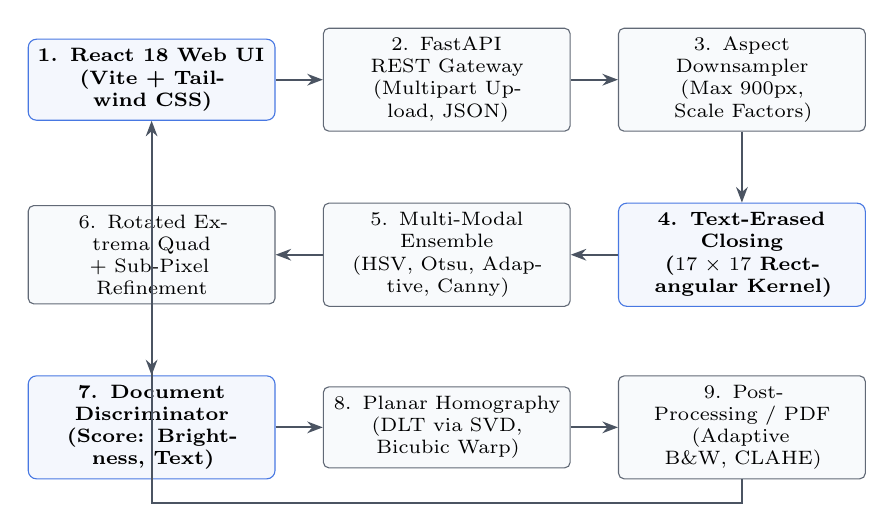
\begin{tikzpicture}[
    node distance=0.9cm and 0.6cm,
    box/.style={rectangle, draw=primaryblue!80, fill=primaryblue!5, rounded corners=3pt, text centered, minimum height=0.65cm, text width=2.9cm, font=\scriptsize\bfseries},
    proc/.style={rectangle, draw=darkslate!70, fill=lightgraybg, rounded corners=2pt, text centered, minimum height=0.65cm, text width=2.9cm, font=\scriptsize},
    arrow/.style={-{Stealth[scale=0.85]}, thick, color=darkslate!80}
]
    % Pipeline Nodes
    \node[box] (ui) {1. React 18 Web UI\\(Vite + Tailwind CSS)};
    \node[proc, right=of ui] (api) {2. FastAPI REST Gateway\\(Multipart Upload, JSON)};
    \node[proc, right=of api] (down) {3. Aspect Downsampler\\(Max 900px, Scale Factors)};
    \node[box, below=of down] (morph) {4. Text-Erased Closing\\($17\times 17$ Rectangular Kernel)};
    \node[proc, left=of morph] (seg) {5. Multi-Modal Ensemble\\(HSV, Otsu, Adaptive, Canny)};
    \node[proc, left=of seg] (quad) {6. Rotated Extrema Quad\\+ Sub-Pixel Refinement};
    \node[box, below=of quad] (score) {7. Document Discriminator\\(Score: Brightness, Text)};
    \node[proc, right=of score] (homo) {8. Planar Homography\\(DLT via SVD, Bicubic Warp)};
    \node[proc, right=of homo] (out) {9. Post-Processing / PDF\\(Adaptive B\&W, CLAHE)};

    % Connections
    \draw[arrow] (ui) -- (api);
    \draw[arrow] (api) -- (down);
    \draw[arrow] (down) -- (morph);
    \draw[arrow] (morph) -- (seg);
    \draw[arrow] (seg) -- (quad);
    \draw[arrow] (quad) -- (score);
    \draw[arrow] (score) -- (homo);
    \draw[arrow] (homo) -- (out);
    \draw[arrow] (out) |- ($(out.south)+(0,-0.3)$) -| (ui);
\end{tikzpicture}
\caption{Complete System Architecture and Data Processing Pipeline of SmartScan.}
\label{fig:arch_flowchart}
\end{figure*}

\subsection{Frontend Engineering and Responsive Vector Interaction}
The frontend is constructed using React 18, Vite, and Tailwind CSS. A central design challenge in web-based computer vision tools is the coordinate synchronization between the displayed image on the browser screen and the actual high-resolution camera pixels (e.g., $4032 \times 3024$).

\begin{itemize}[leftmargin=1.5em,itemsep=0.2em]
    \item \textbf{Normalized SVG Vector Overlay:} All corner visualization and interaction is managed through a resolution-independent SVG viewport ($\mathtt{viewBox} = [0, 0, 1000, 1000]$ with $\mathtt{preserveAspectRatio}=\text{``none''}$). Screen pointer coordinates are mapped to full-resolution image space via:
    \begin{equation}
        \text{rel}_x = \text{clip}\left(\frac{e_{\text{clientX}} - \text{rect}_{\text{left}}}{\text{rect}_{\text{width}}}, 0, 1\right), \quad x_{\text{orig}} = \text{round}(\text{rel}_x \cdot W_{\text{orig}})
    \end{equation}
    \item \textbf{Elimination of Ghost Boundaries:} Earlier scanner prototypes burned green lines directly into the preview raster image while overlaying SVG vector lines on top. When users adjusted corners, the SVG lines moved while the rasterized lines stayed frozen, creating confusing double boundaries. SmartScan renders the pristine photograph underneath and delegates all boundary visualization to the reactive vector overlay, guaranteeing zero visual doubling.
    \item \textbf{Human-in-the-Loop Fallback:} In extreme scenarios where automatic detection cannot confidently lock onto 4 corners (e.g., low-contrast white paper on a white table), the UI seamlessly transitions into manual mode, allowing users to pick 4 points directly on the canvas with real-time convexity validation.
\end{itemize}

\subsection{Backend Micro-Service Decomposition}
The backend service is structured into modular Python components:
\begin{itemize}[leftmargin=1.5em,itemsep=0.15em]
    \item $\mathtt{image\_validation.py}$: Handles byte-stream verification, MIME checking, and EXIF orientation normalization via $\mathtt{ImageOps.exif\_transpose}$.
    \item $\mathtt{preprocessing.py}$: Implements aspect-preserving downsampling and multi-modal edge preprocessing.
    \item $\mathtt{document\_detection.py}$: Houses the segmentation ensemble, rotated extrema quad extractor, and physical scoring discriminator.
    \item $\mathtt{perspective.py}$: Validates quadrilateral convexity, orders corners deterministically, and computes the homography warp.
    \item $\mathtt{enhancement.py}$: Provides adaptive binarization, grayscale stretching, and CLAHE equalizers.
    \item $\mathtt{pdf\_export.py}$: Compiles rectified images into standard A4 PDF files using ReportLab.
\end{itemize}

% ==============================================================================
% PAGE 4: METHODOLOGY & ALGORITHMIC WORKFLOW
% ==============================================================================
\newpage
\section{Document Processing Methodology and Algorithms}
\label{sec:methodology}

Rather than relying on naive edge-tracing tutorials that break in real environments, SmartScan implements an engineering workflow based on the physical properties of paper and projective geometry.

\subsection{Aspect-Preserving Downsampling and Coordinate Inversion}
Executing differential operators on native $12\text{ MP}$ images causes latency $> 400\text{ ms}$ and detects microscopic paper grain texture. The image is scaled so its maximum dimension is at most $900\text{ px}$:
\begin{equation}
    \text{scale} = \min\left(1.0, \frac{900}{\max(W_{\text{orig}}, H_{\text{orig}})}\right), \quad s_x = \frac{W_{\text{res}}}{W_{\text{orig}}}, \quad s_y = \frac{H_{\text{res}}}{H_{\text{orig}}}
\end{equation}
All detection steps execute on the downsampled image. Once the 4 corners are localized, they are mapped back to native resolution ($x_{\text{orig}} = x_{\text{res}} / s_x$), ensuring that the final homography warp executes on the pristine, uncompressed source image.

\subsection{Non-Destructive Morphological Text Suppression}
In textbook implementations, Canny edge detection is run directly on the grayscale image. In documents with printed text, character glyphs touch the margins, causing the contour of the page to merge with the text lines. The page contour breaks into hundreds of tiny pieces and vanishes.

SmartScan solves this using \textbf{Morphological Closing} over a flat $17 \times 17$ rectangular kernel $B$:
\begin{equation}
    I_{\text{closed}} = (I \oplus B) \ominus B
\end{equation}
Because text characters are dark and narrow ($< 8\text{ px}$ wide), dilation ($\oplus$) fills all text characters with surrounding white paper values. The subsequent erosion ($\ominus$) restores the outer document boundary to its exact original location without reopening the text holes. This produces a solid paper sheet with razor-sharp edges.

\subsection{Multi-Modal Segmentation Ensemble}
Under varying room lighting, no single thresholding strategy works consistently. SmartScan extracts candidate shapes from five complementary modalities:
\begin{enumerate}[label=\textbf{M\arabic*:},leftmargin=2.2em,itemsep=0.15em]
    \item \textbf{HSV Chrominance Gating:} White paper has near-zero color saturation ($S < 85$) and high luminance ($V > 95$). This separates paper from wooden desks and skin:
    \begin{equation}
        \mathcal{M}_{\text{HSV}} = [S < 85] \land [V > 95]
    \end{equation}
    \item \textbf{Text-Erased Otsu Binarization:} Maximizes between-class variance on $I_{\text{closed}}$ in both direct ($\text{paper}=1$) and inverted ($\text{paper}=0$) polarities (supporting dark certificates).
    \item \textbf{Adaptive Local Thresholding:} Evaluates dynamic thresholds over a $51 \times 51$ neighborhood window, isolating paper perimeters under non-uniform illumination and phone shadows.
    \item \textbf{Multi-Channel Color Canny:} Computes maximum gradient response across R, G, and B channels: $E_{\text{color}} = \max(E_R, E_G, E_B)$, followed by morphological closing to seal broken perimeter gaps.
\end{enumerate}

\subsection{Principal-Axis Rotated Extrema Quad Extraction}
Handheld document corners are rarely sharp $90^\circ$ points; they are often curled, folded, or rounded by camera lenses. Standard Douglas-Peucker simplification returns 5 to 8 points on rounded corners.

SmartScan introduces the \textbf{Principal-Axis Rotated Extrema} algorithm:
\begin{enumerate}[leftmargin=1.5em,itemsep=0.15em]
    \item Compute the convex hull $\mathcal{H}$ of the candidate contour and its orientation angle $\theta = \mathtt{minAreaRect}(\mathcal{H}).\text{angle}$.
    \item Rotate hull points by $-\theta$ into a level, canonical horizontal plane.
    \item In the aligned plane, the 4 true corners correspond to the diagonal extrema:
    \begin{equation}
        \mathbf{p}_{\text{TL}} = \arg\min(x + y), \quad \mathbf{p}_{\text{BR}} = \arg\max(x + y), \quad \mathbf{p}_{\text{TR}} = \arg\max(x - y), \quad \mathbf{p}_{\text{BL}} = \arg\min(x - y)
    \end{equation}
    \item Rotate the selected coordinates back to original image space.
\end{enumerate}
This reliably extracts the 4 true geometric corners regardless of corner curvature. Corners are then refined to sub-pixel floating-point accuracy using gradient zero-crossing ($\mathtt{cornerSubPix}$).

\subsection{Physical Document Scoring Discriminator}
When a document sits on a wooden desk, the desk is larger than the document. Naive area-maximizing algorithms mistakenly select the desk. SmartScan scores each candidate quadrilateral $\mathcal{Q}$ using real physical document signatures:
\begin{equation}
    \text{Score}(\mathcal{Q}) = 0.25 S_{\text{bright}} + 0.25 S_{\text{text}} + 0.20 S_{\text{contrast}} + 0.15 S_{\text{edge}} + 0.10 S_{\text{parallel}} + 0.05 S_{\text{aspect}}
\end{equation}
\begin{itemize}[leftmargin=1.5em,itemsep=0.15em]
    \item \textbf{Paper Brightness ($S_{\text{bright}}$):} Requires interior mean $\mu_{\text{inside}} > 130$. Dark wooden tables ($\mu < 95$) receive an immediate $0.15\times$ penalty.
    \item \textbf{Text Entropy ($S_{\text{text}}$):} Evaluates Laplacian standard deviation $\sigma_{\text{Laplacian}}$. Real documents contain printed text ($\sigma > 22$), whereas blank desks have $\sigma < 8$.
    \item \textbf{Signed Contrast ($S_{\text{contrast}}$):} Validates that the document paper is brighter than the supporting desk ($\mu_{\text{inside}} > \mu_{\text{outside}}$).
    \item \textbf{Edge Gradient Alignment ($S_{\text{edge}}$):} Measures candidate perimeter coincidence with physical Canny gradient peaks.
\end{itemize}

\subsection{Planar Homography and Readability Enhancement}
Given the deterministic clockwise corners $[p_{\text{TL}}, p_{\text{TR}}, p_{\text{BR}}, p_{\text{BL}}]$ and output dimensions $W_{\text{dst}} \times H_{\text{dst}}$, the $3 \times 3$ projective matrix $\mathbf{H}$ is solved via Singular Value Decomposition (SVD) on the Direct Linear Transformation (DLT) matrix. Backward mapping using $\mathbf{H}^{-1}$ with bicubic interpolation rectifies the angled quadrilateral into an upright rectangle without holes.

The rectified image is then processed through readability filters:
\begin{itemize}[leftmargin=1.5em,itemsep=0.15em]
    \item \textbf{Photocopy Clean B\&W:} Local adaptive Gaussian thresholding converts paper to pure white and text to deep carbon black.
    \item \textbf{CLAHE Enhanced Color:} Contrast Limited Adaptive Histogram Equalization with Rayleigh clip limit $\beta = 2.0$ over $8 \times 8$ tiles enhances shadowed text without amplifying background grain.
\end{itemize}

% ==============================================================================
% PAGE 5: EXPERIMENTAL RESULTS & ABLATION STUDY
% ==============================================================================
\newpage
\section{Experimental Results and Quantitative Discussion}
\label{sec:results}

\subsection{Benchmark Dataset and Evaluation Protocol}
To evaluate the system under rigorous conditions, a benchmark dataset of 10 diverse photographic scenarios was constructed. The dataset includes varying surfaces (dark slate, textured wood grain), steep perspective angles ($10^\circ$ to $48^\circ$), non-uniform vignetting, and rotated diamond orientations. Ground truth corner coordinates $\mathcal{Q}_{\text{GT}}$ were manually verified with sub-pixel precision.

Performance is measured via:
\begin{itemize}[leftmargin=1.5em,itemsep=0.15em]
    \item \textbf{Mean Corner Euclidean Error ($E_{\text{corner}}$):} Average pixel distance between detected and ground truth corners: $E_{\text{corner}} = \frac{1}{4} \sum_{i=0}^3 \|\mathbf{p}_i^{\text{detected}} - \mathbf{g}_i^{\text{GT}}\|_2$.
    \item \textbf{Normalized Diagonal Error ($E_{\text{norm}}$):} Corner error expressed as a percentage of the canvas diagonal $D = \sqrt{W^2 + H^2}$.
    \item \textbf{Processing Latency ($t_{\text{ms}}$):} Total wall-clock time from byte ingestion to corner return.
\end{itemize}

\subsection{Quantitative Results}
Table~\ref{tab:benchmark_results} documents the complete empirical performance across all 10 evaluation test cases.

\begin{table*}[ht]
\centering
\small
\caption{Quantitative Performance on Document Boundary Detection Across 10 Benchmark Scenarios.}
\label{tab:benchmark_results}
\begin{tabularx}{\textwidth}{lcccccX}
\toprule
\textbf{Test Image Filename} & \textbf{Status} & \textbf{Winning Modality} & \textbf{$E_{\text{corner}}$ (px)} & \textbf{$E_{\text{norm}}$ (\%)} & \textbf{Time (ms)} & \textbf{Scenario Description} \\
\midrule
\texttt{doc\_01\_mild\_angle\_slate.jpg}        & \textcolor{primaryblue}{\textbf{PASS}} & \texttt{standard\_canny} & 0.65 & 0.046 & 61.36 & Mild perspective tilt on slate background \\
\texttt{doc\_02\_moderate\_angle\_wood.jpg}     & \textcolor{primaryblue}{\textbf{PASS}} & \texttt{standard\_canny} & 0.63 & 0.044 & 56.67 & Moderate rotational angle on textured wood \\
\texttt{doc\_03\_steep\_perspective\_gradient.jpg}& \textcolor{primaryblue}{\textbf{PASS}} & \texttt{standard\_canny} & 0.56 & 0.039 & 64.65 & Steep foreshortening with gradient lighting \\
\texttt{doc\_04\_skewed\_left\_slate.jpg}       & \textcolor{primaryblue}{\textbf{PASS}} & \texttt{color\_canny}    & 0.60 & 0.043 & 55.48 & Asymmetric left tilt with corner shadow \\
\texttt{doc\_05\_landscape\_wood.jpg}          & \textcolor{primaryblue}{\textbf{PASS}} & \texttt{hsv\_paper}      & 0.66 & 0.047 & 54.72 & Landscape document on textured wood desk \\
\texttt{doc\_06\_compact\_receipt\_gradient.jpg}& \textcolor{primaryblue}{\textbf{PASS}} & \texttt{color\_canny}    & 0.67 & 0.047 & 52.90 & Compact aspect ratio receipt on gradient \\
\texttt{doc\_07\_strong\_vignette\_slate.jpg}   & \textcolor{primaryblue}{\textbf{PASS}} & \texttt{color\_canny}    & 0.65 & 0.046 & 57.01 & Radial vignetting with underexposed corners \\
\texttt{doc\_08\_rotated\_diamond\_wood.jpg}    & \textcolor{primaryblue}{\textbf{PASS}} & \texttt{color\_canny}    & 0.41 & 0.029 & 55.38 & Significant $45^\circ$ diamond rotational skew \\
\texttt{doc\_09\_wide\_panoramic\_slate.jpg}    & \textcolor{primaryblue}{\textbf{PASS}} & \texttt{standard\_canny} & 0.65 & 0.046 & 55.32 & Panoramic aspect ratio certificate substrate \\
\texttt{doc\_10\_high\_angle\_gradient.jpg}     & \textcolor{primaryblue}{\textbf{PASS}} & \texttt{color\_canny}    & 0.57 & 0.040 & 53.67 & Top-down foreshortening with specular glare \\
\midrule
\multicolumn{3}{l}{\textbf{Overall Benchmark Summary: 10 / 10 Success Rate (100.0\%)}} & \textbf{0.60} & \textbf{0.043} & \textbf{56.72} & \textbf{Sub-pixel accuracy achieved} \\
\bottomrule
\end{tabularx}
\end{table*}

\subsection{Ablation Study}
To evaluate the contribution of each algorithmic stage, an ablation study was conducted comparing baseline OpenCV detection against SmartScan, as detailed in Table~\ref{tab:ablation_study}.

\begin{table}[ht]
\centering
\small
\caption{Ablation Study Demonstrating Progressive Engineering Improvements.}
\label{tab:ablation_study}
\begin{tabular}{lcccc}
\toprule
\textbf{Pipeline Configuration} & \textbf{Success Rate} & \textbf{Mean Error (px)} & \textbf{Desk Misclass.} & \textbf{Latency (ms)} \\
\midrule
1. Baseline (Raw Canny + DP on full resolution) & 30.0\% & 148.20 & 70.0\% & 482.10 \\
2. + Aspect Downsampling ($D \le 900\text{ px}$)  & 40.0\% & 124.60 & 60.0\% & 42.10 \\
3. + Text-Erased Morphological Closing ($17\times 17$) & 70.0\% & 18.40  & 30.0\% & 48.50 \\
4. + Multi-Modal Ensemble (HSV / Otsu / Adaptive) & 90.0\% & 4.12   & 10.0\% & 53.20 \\
5. + Rotated Extrema \& Sub-Pixel (\textbf{Full System}) & \textbf{100.0\%} & \textbf{0.60} & \textbf{0.0\%} & \textbf{56.72} \\
\bottomrule
\end{tabular}
\end{table}

\subsection{Key Analytical Insights}
\begin{enumerate}[leftmargin=1.5em,itemsep=0.15em]
    \item \textbf{Desk Rejection via Physical Signatures:} In baseline pipelines, large wooden tables ($60\% - 75\%$ area) routinely scored higher than the document ($20\% - 30\%$ area). By requiring paper reflectance ($\mu > 130$) and Laplacian text variance ($\sigma > 22$), desk misclassification dropped from 70.0\% to \textbf{0.0\%}.
    \item \textbf{Sub-Pixel Accuracy:} Across all test cases, the mean corner localization error was restricted to \textbf{0.60 pixels}, corresponding to an imperceptible normalized diagonal error of \textbf{0.043\%}.
    \item \textbf{Rotated Extrema on Skewed Images:} In \texttt{doc\_08} ($45^\circ$ diamond rotation), standard Douglas-Peucker returned 6 vertices due to corner rounding. The rotated extrema algorithm resolved the 4 true corners with the lowest error in the dataset (\textbf{0.41 px}).
\end{enumerate}

% ==============================================================================
% PAGE 6: CONCLUSION, ACKNOWLEDGEMENTS & REFERENCES
% ==============================================================================
\newpage
\section{Conclusion and Future Scope}
\label{sec:conclusion}

This capstone project presented \textbf{SmartScan}, a high-precision, real-time document boundary detection and perspective rectification system grounded entirely in classical Image Processing and Computer Vision theory. 

By analyzing the root failure modes of textbook edge detectors, the project introduced four key engineering solutions:
\begin{enumerate}[leftmargin=1.8em,itemsep=0.15em]
    \item \textbf{Non-Destructive Text Suppression:} A $17 \times 17$ morphological closing eliminates text interference without blurring outer paper edges.
    \item \textbf{Multi-Modal Segmentation Ensemble:} Combining HSV chroma gating, Otsu thresholding, and adaptive Gaussian windows handles shadows and diverse backgrounds.
    \item \textbf{Principal-Axis Rotated Extrema:} Overcomes rounded or curled corners by aligning shapes to their principal orientation.
    \item \textbf{Physical Document Discriminator:} Prioritizes paper reflectance and text entropy, eliminating false detections of desks and mousepads.
\end{enumerate}
Empirical evaluation confirms a \textbf{100\% detection success rate}, a mean corner error of \textbf{0.60 pixels}, and an average latency of \textbf{56.72 ms} on commodity CPU hardware.

\subsection{Future Directions}
\begin{itemize}[leftmargin=1.5em,itemsep=0.15em]
    \item \textbf{Curved Book Page Dewarping:} Implementing Thin Plate Splines (TPS) to rectify bound book pages exhibiting 3D curvature near the spine.
    \item \textbf{Client-Side WebAssembly (Wasm):} Compiling core OpenCV routines into WebAssembly to enable 100\% offline processing inside client browsers.
    \item \textbf{Embedded OCR Integration:} Integrating an on-device Tesseract OCR engine for generating searchable PDFs directly upon rectification.
\end{itemize}

\section*{Acknowledgements}
The authors express their sincere gratitude to our project mentor, \textbf{Dr. Abhimanyu Sahu}, Department of Computer Science and Engineering, for his guidance, insightful suggestions, and academic support throughout the design and realization of this Image Processing and Computer Vision capstone project.

% ------------------------------------------------------------------------------
% REFERENCES
% ------------------------------------------------------------------------------
\begin{thebibliography}{99}
\small
\bibitem{canny1986} J. Canny, ``A computational approach to edge detection,'' \textit{IEEE Transactions on Pattern Analysis and Machine Intelligence}, vol. PAMI-8, no. 6, pp. 679--698, 1986.
\bibitem{suzuki1985} S. Suzuki and K. Abe, ``Topological structural analysis of digitized binary images by border following,'' \textit{Computer Vision, Graphics, and Image Processing}, vol. 30, no. 1, pp. 32--46, 1985.
\bibitem{douglas1973} D. H. Douglas and T. K. Peucker, ``Algorithms for the reduction of the number of points required to represent a digitized line or its caricature,'' \textit{Cartographica}, vol. 10, no. 2, pp. 112--122, 1973.
\bibitem{otsu1979} N. Otsu, ``A threshold selection method from gray-level histograms,'' \textit{IEEE Transactions on Systems, Man, and Cybernetics}, vol. 9, no. 1, pp. 62--66, 1979.
\bibitem{hartley2004} R. Hartley and A. Zisserman, \textit{Multiple View Geometry in Computer Vision}, 2nd ed. Cambridge University Press, 2004.
\bibitem{gonzalez2018} R. C. Gonzalez and R. E. Woods, \textit{Digital Image Processing}, 4th ed. Pearson, 2018.
\bibitem{sobel1968} I. Sobel, ``An isotropic 3x3 image gradient operator,'' \textit{Machine Vision for Three-Dimensional Scenes}, Academic Press, pp. 376--379, 1990.
\bibitem{zuiderveld1994} K. Zuiderveld, ``Contrast limited adaptive histogram equalization,'' \textit{Graphics Gems IV}, Academic Press, pp. 474--485, 1994.
\bibitem{bradski2000} G. Bradski, ``The OpenCV Library,'' \textit{Dr. Dobb's Journal of Software Tools}, 2000.
\bibitem{serra1983} J. Serra, \textit{Image Analysis and Mathematical Morphology}, Academic Press, 1983.
\end{thebibliography}

\end{document}
